\documentclass[10pt]{beamer}
\usepackage[utf8]{inputenc}
\usepackage{hyperref}
\usepackage[scaled]{helvet}
\usepackage[T1]{fontenc}
\usetheme{Berkeley}
\beamertemplatenavigationsymbolsempty
\setbeamertemplate{headline}{}
\setbeamersize{sidebar width left=1.5cm}
\setbeamerfont{section in sidebar}{size=\fontsize{6}{6}\selectfont}
\setbeamerfont{title in sidebar}{size=\fontsize{6}{6}\selectfont}
\title{Tracing in FoodChain-Lab}
\date{}

\begin{document}
\maketitle

\section{Topics}
\begin{frame}
\leftskip1em\textbf{Learn}
	\begin{itemize}
		\item to visualise forward and backward traces of a station in the Tracing View
		\item to deactivate “Cross Contamination” and how this changes the trace
	\end{itemize}
\end{frame}

\section{1a}
\begin{frame}
	\begin{center}
  		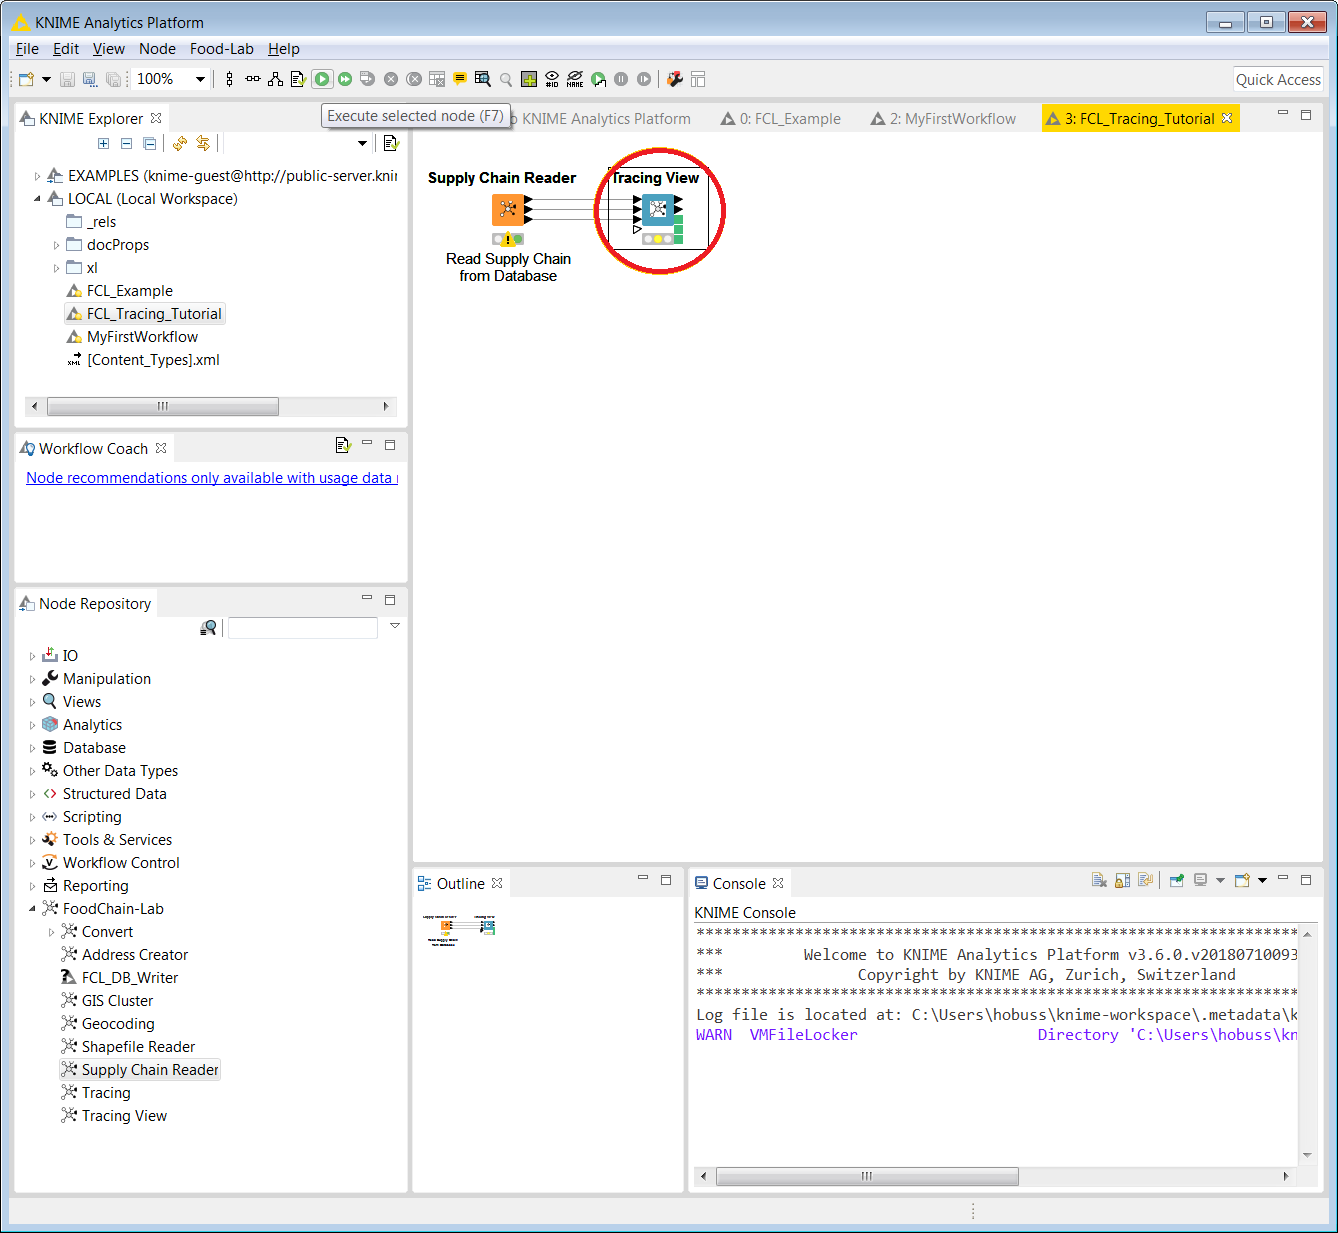
\includegraphics[height=0.6\textheight]{1a.png}
	\end{center}
	\begin{itemize}
		\item Import the Example Workflow from \url{https://github.com/SiLeBAT/BfROpenLabResources/raw/master/GitHubPages/workflows/FCL_Tracing_Tutorial.knwf}.
		\item Open the \textbf{Tracing View} by double-clicking on it.
	\end{itemize}
\end{frame}

\section{1b}
\begin{frame}
	\begin{center}
  		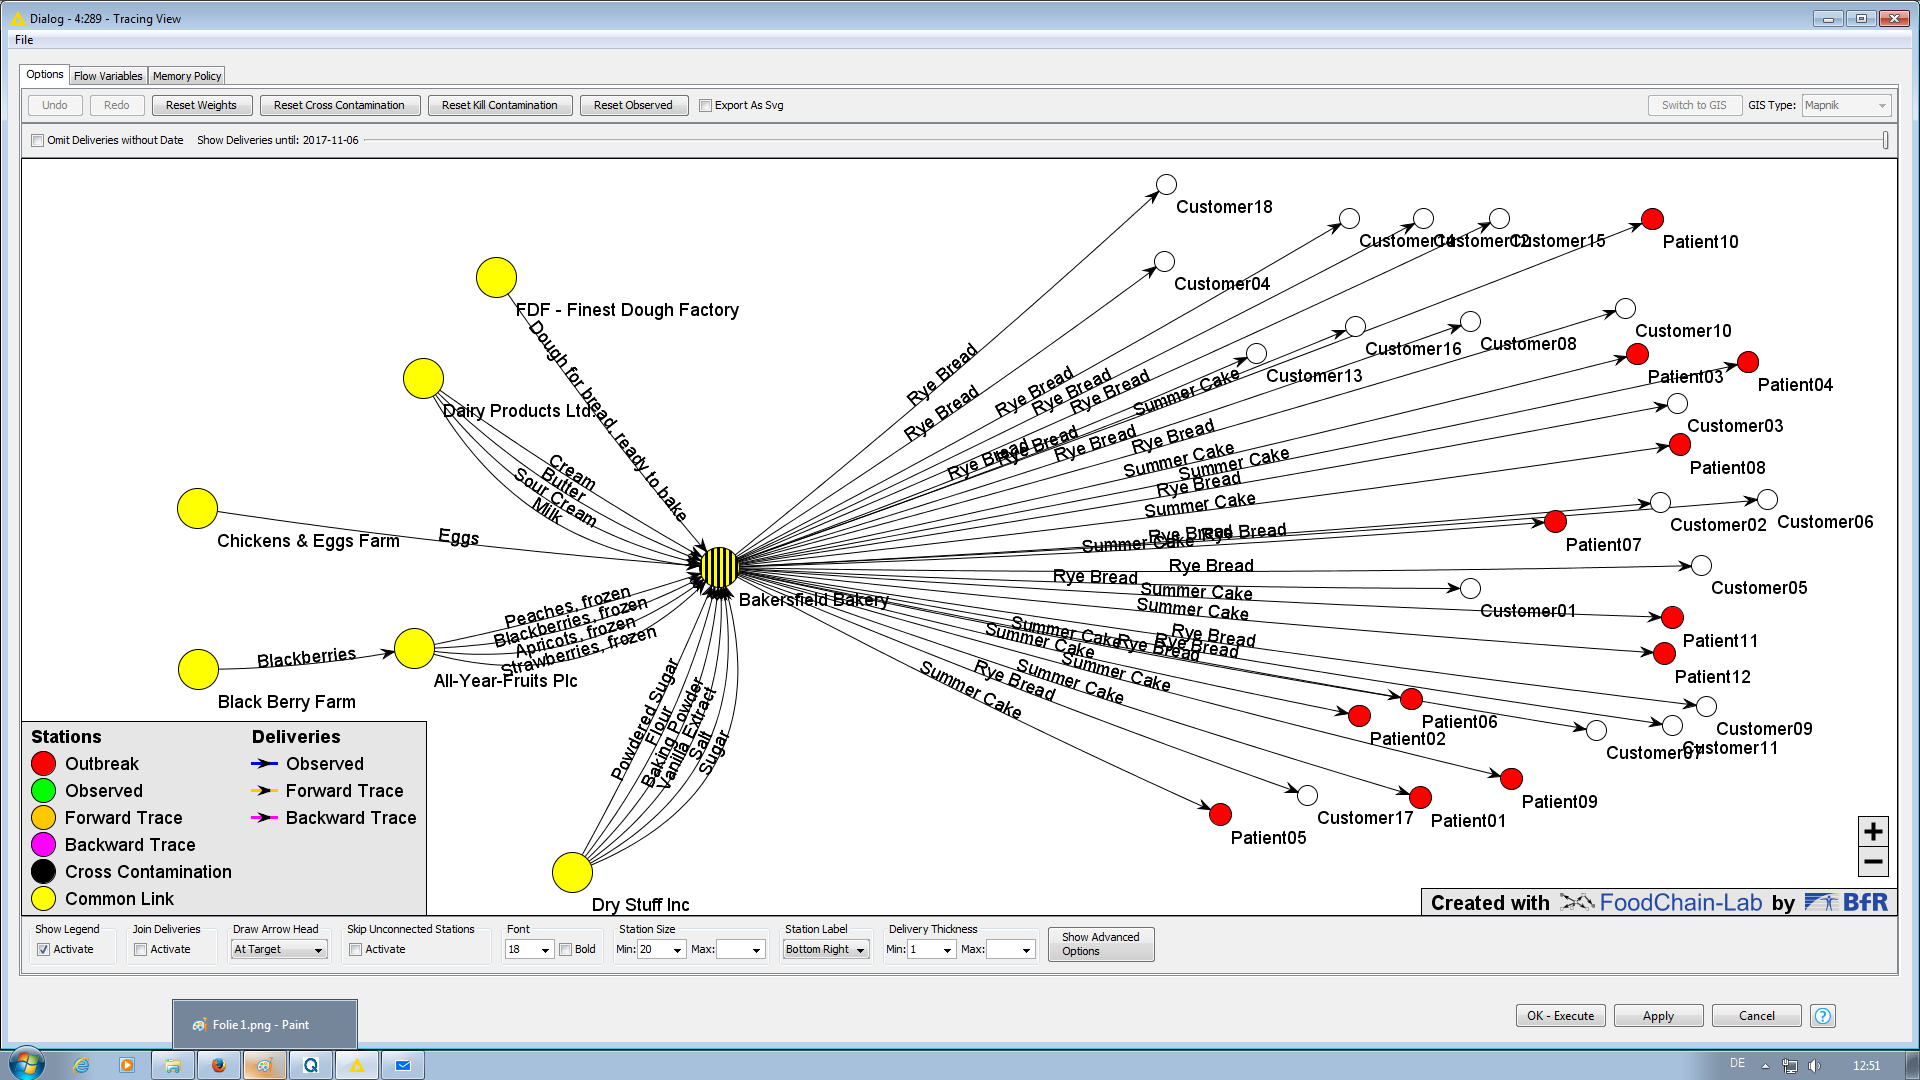
\includegraphics[height=0.6\textheight]{1b.png}
	\end{center}
	\begin{itemize}
		\item In the delivery graph you can see 12 outbreak stations (red), six stations which are connected to outbreak stations and are thus a common link (yellow) and one station (the Bakersfield Bakery) which is both a common link (yellow) and in which also cross contamination is assumed (black).
	\end{itemize}
\end{frame}

\section{1c}
\begin{frame}
	\begin{itemize}
		\item To show two properties, stations are striped. Here, the Bakersfield bakery is striped  black and yellow.
		\item The size of each station is based on its ``Score'', which depends on the outbreak stations that are connected to each station.
		\item In this scenario, the outbreak stations are people. They have bought a product which was contaminated and they became ill. We want to find out, where the source of the contamination is. But do we already know enough to solve the riddle \textit{in silico}?
	\end{itemize}
\end{frame}

\section{2}
\begin{frame}
	\begin{center}
  		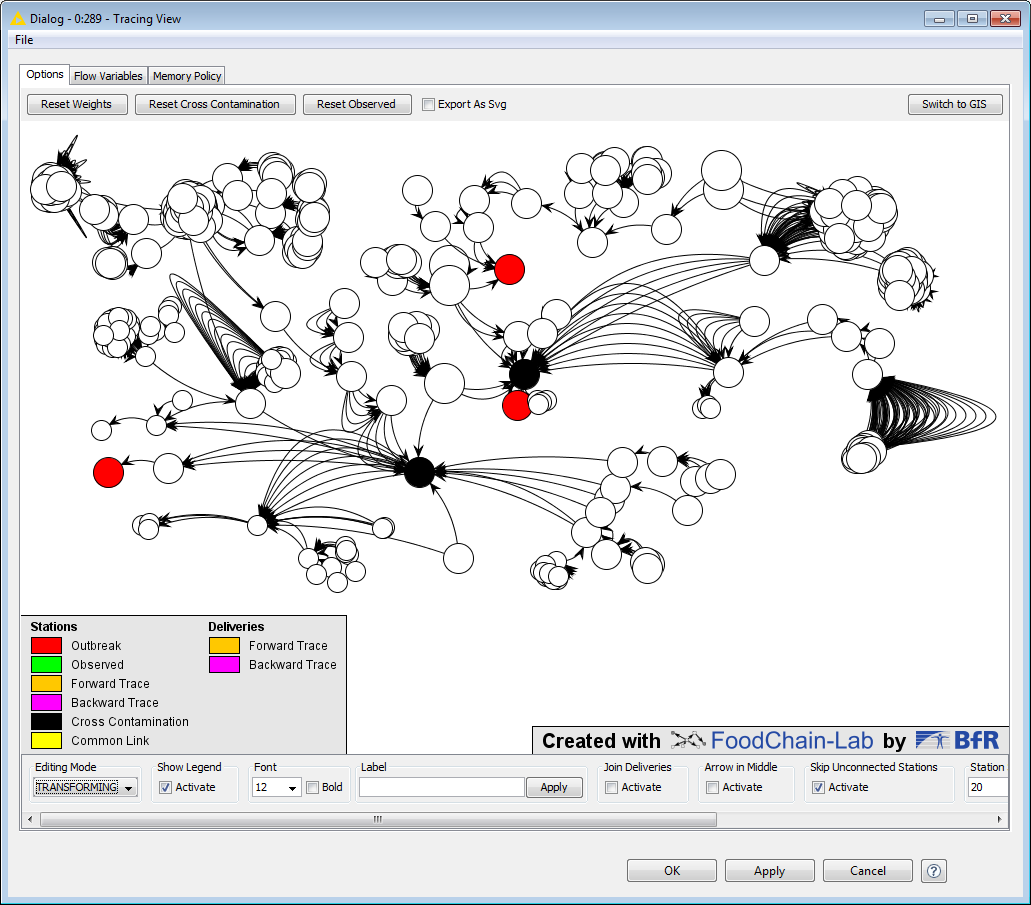
\includegraphics[height=0.6\textheight]{2.png}
	\end{center}
	\begin{itemize}
		\item There is a suspicion that \textit{All-Year-Fruits Plc} has supplied contaminated products. We will now observe the trace of this station in detail. We would like to see whether the company’s forward trace reaches the outbreak stations.
		\item Double click on the station \textit{All-Year-Fruits Plc} in the red circle.
	\end{itemize}
\end{frame}

\section{3a}
\begin{frame}
	\begin{center}
  		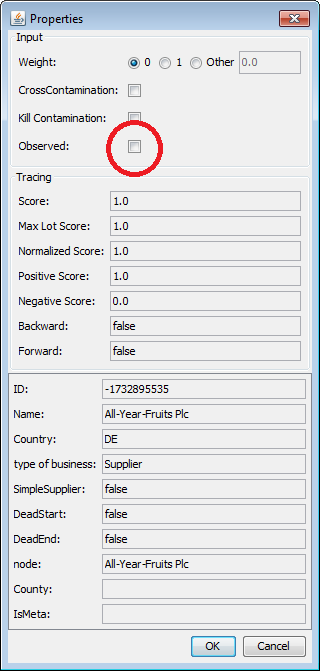
\includegraphics[height=0.6\textheight]{3a.png}
	\end{center}
	\begin{itemize}
		\item A dialog will pop up, showing all attributes of the station.
		\item Additionally, it is possible to change ``Weight'', ``Cross Contamination'', ``Kill Contamination'' and ``Observed''.
		\item Select ``Observed'' and press OK.
	\end{itemize}
\end{frame}

\section{3b}
\begin{frame}
	\begin{center}
  		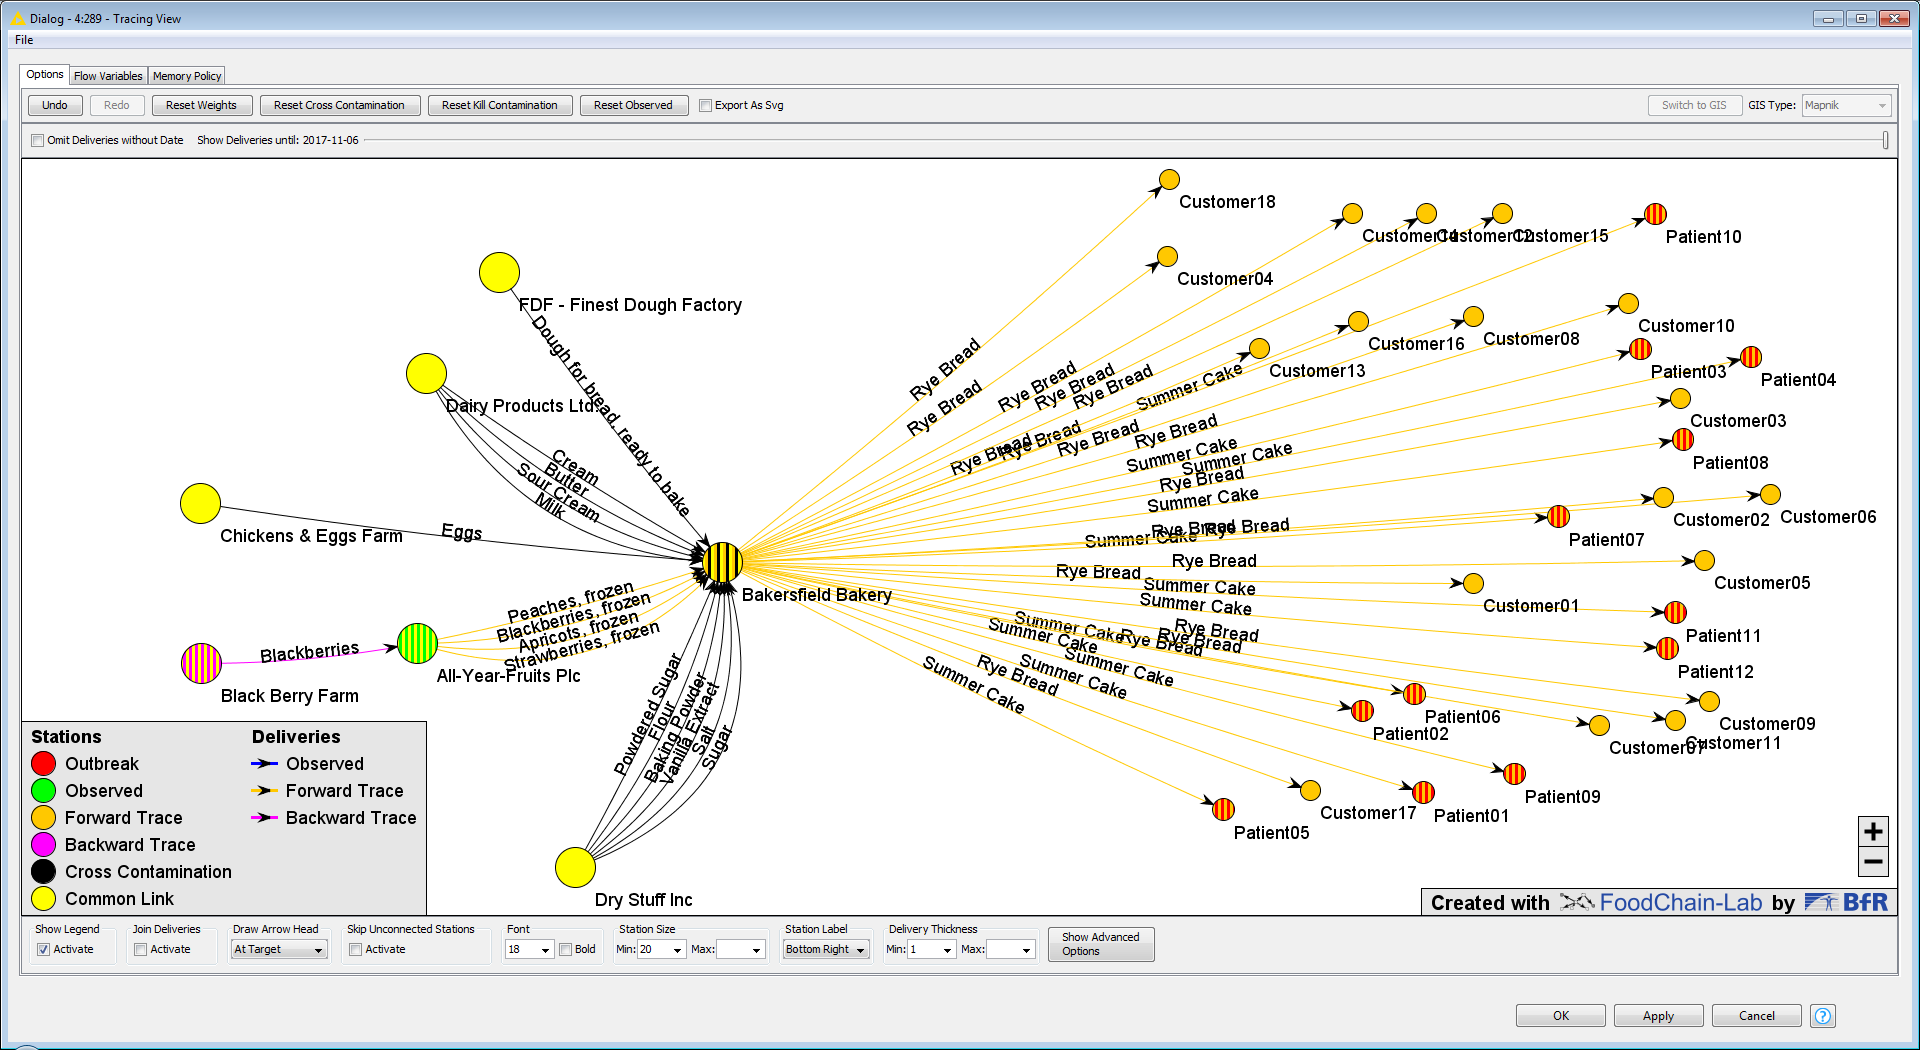
\includegraphics[height=0.6\textheight]{3b.png}
	\end{center}
	\begin{itemize}
		\item Stations and deliveries on the forward trace are orange and the ones of the backward trace are purple. The observed station is green.
		\item The outbreak stations (here: patients) are striped red and orange now. This means they really are on the forward trace of the observed station.
	\end{itemize}
\end{frame}

\section{4}
\begin{frame}
	\begin{center}
  		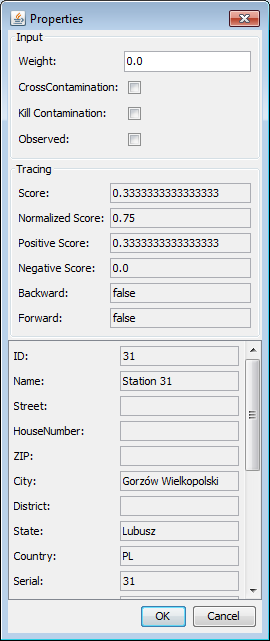
\includegraphics[height=0.6\textheight]{4.png}
	\end{center}
	\begin{itemize}
		\item However, also stations for which no outbreak was confirmed are on the forward trace (here: customers).
		\item Perhaps there was one assumption to many. What happens if we deactivate ``cross contamination'' in the station in the red circle? Double click this station.
	\end{itemize}
\end{frame}

\section{5a}
\begin{frame}
	\begin{center}
  		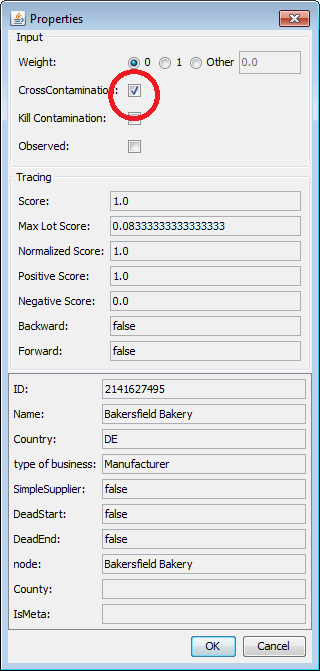
\includegraphics[height=0.6\textheight]{5a.png}
	\end{center}
	\begin{itemize}
		\item Uncheck ``CrossContamination''. This means we assume that even if contaminated products were used by the bakery the contamination coming from one ingredient did not spread to all of the bakery’s products but only to those that contain this ingredient. Press OK.
	\end{itemize}
\end{frame}

\section{5b}
\begin{frame}
	\begin{center}
  		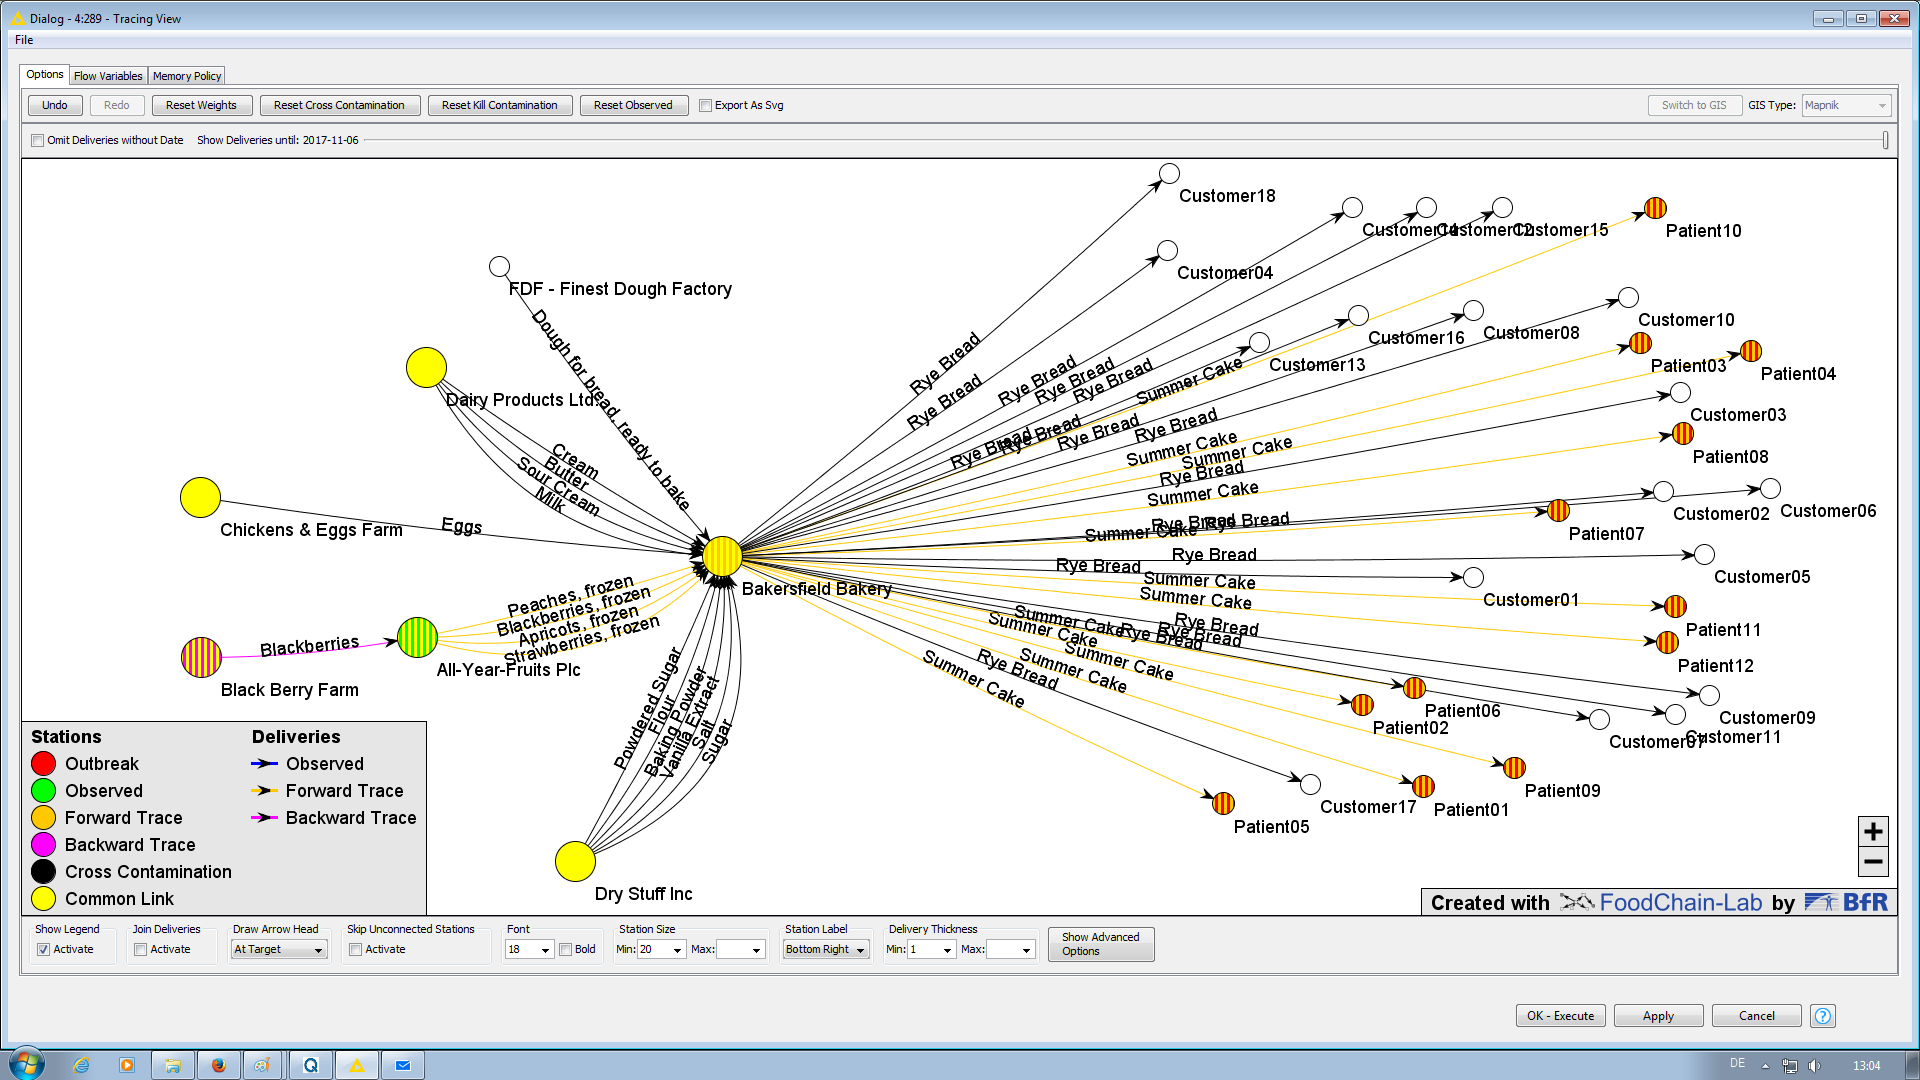
\includegraphics[height=0.6\textheight]{5b.png}
	\end{center}
	\begin{itemize}
		\item Deactivating cross contamination changed the forward trace of the observed station.
		\item Now, only the outbreak stations belong to the forward trace.
	\end{itemize}
\end{frame}

\section{5c}
\begin{frame}
	\begin{itemize}
		\item But is All-Year-Fruits Plc the only possible source for contaminated products? Deselect “Observed” in this station and try one of the other common links.
		\item Also other companies might be the source of the contamination. Thus, it is not yet proven that All-Year-Fruits Plc delivered contaminated products.
		\item Perhaps it is time to take samples in these companies…
		\item Some days later you get the results from the laboratory. There was a high bacterial count in a milk pasteurizing machine from Dairy Products Ltd. as well as in milk cartons filled by this company with “pasteurized” milk. The outbreak strain and the strain found in the milk pasteurizer are identical.
	\end{itemize}
\end{frame}

\section{6}
\begin{frame}
	\begin{center}
  		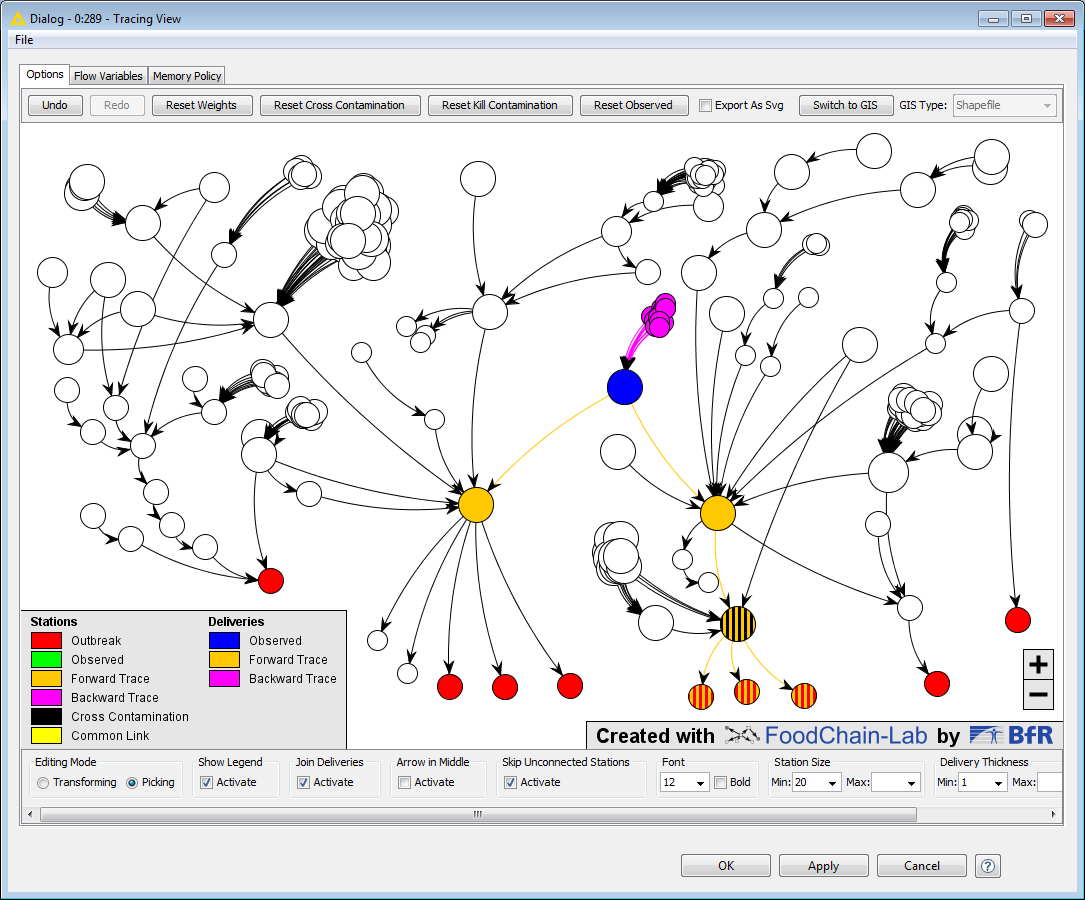
\includegraphics[height=0.6\textheight]{6.png}
	\end{center}
	\begin{itemize}
		\item Uncheck “Observed” in the stations. The Tracing View should look like the screenshot above.
		\item Double click the delivery arrow of the milk (see red oval).
	\end{itemize}
\end{frame}

\section{7a}
\begin{frame}
	\begin{center}
			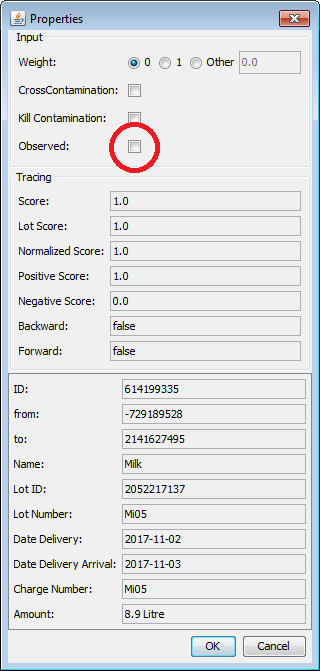
\includegraphics[height=0.6\textheight]{7a.png}
	\end{center}
	\begin{itemize}
		\item Check “Observed” to see the backward and forward traces of the milk which is an ingredient of the Summer Cake consumed by all patients. Press OK.
	\end{itemize}
\end{frame}

\section{7b}
\begin{frame}
	\begin{center}
			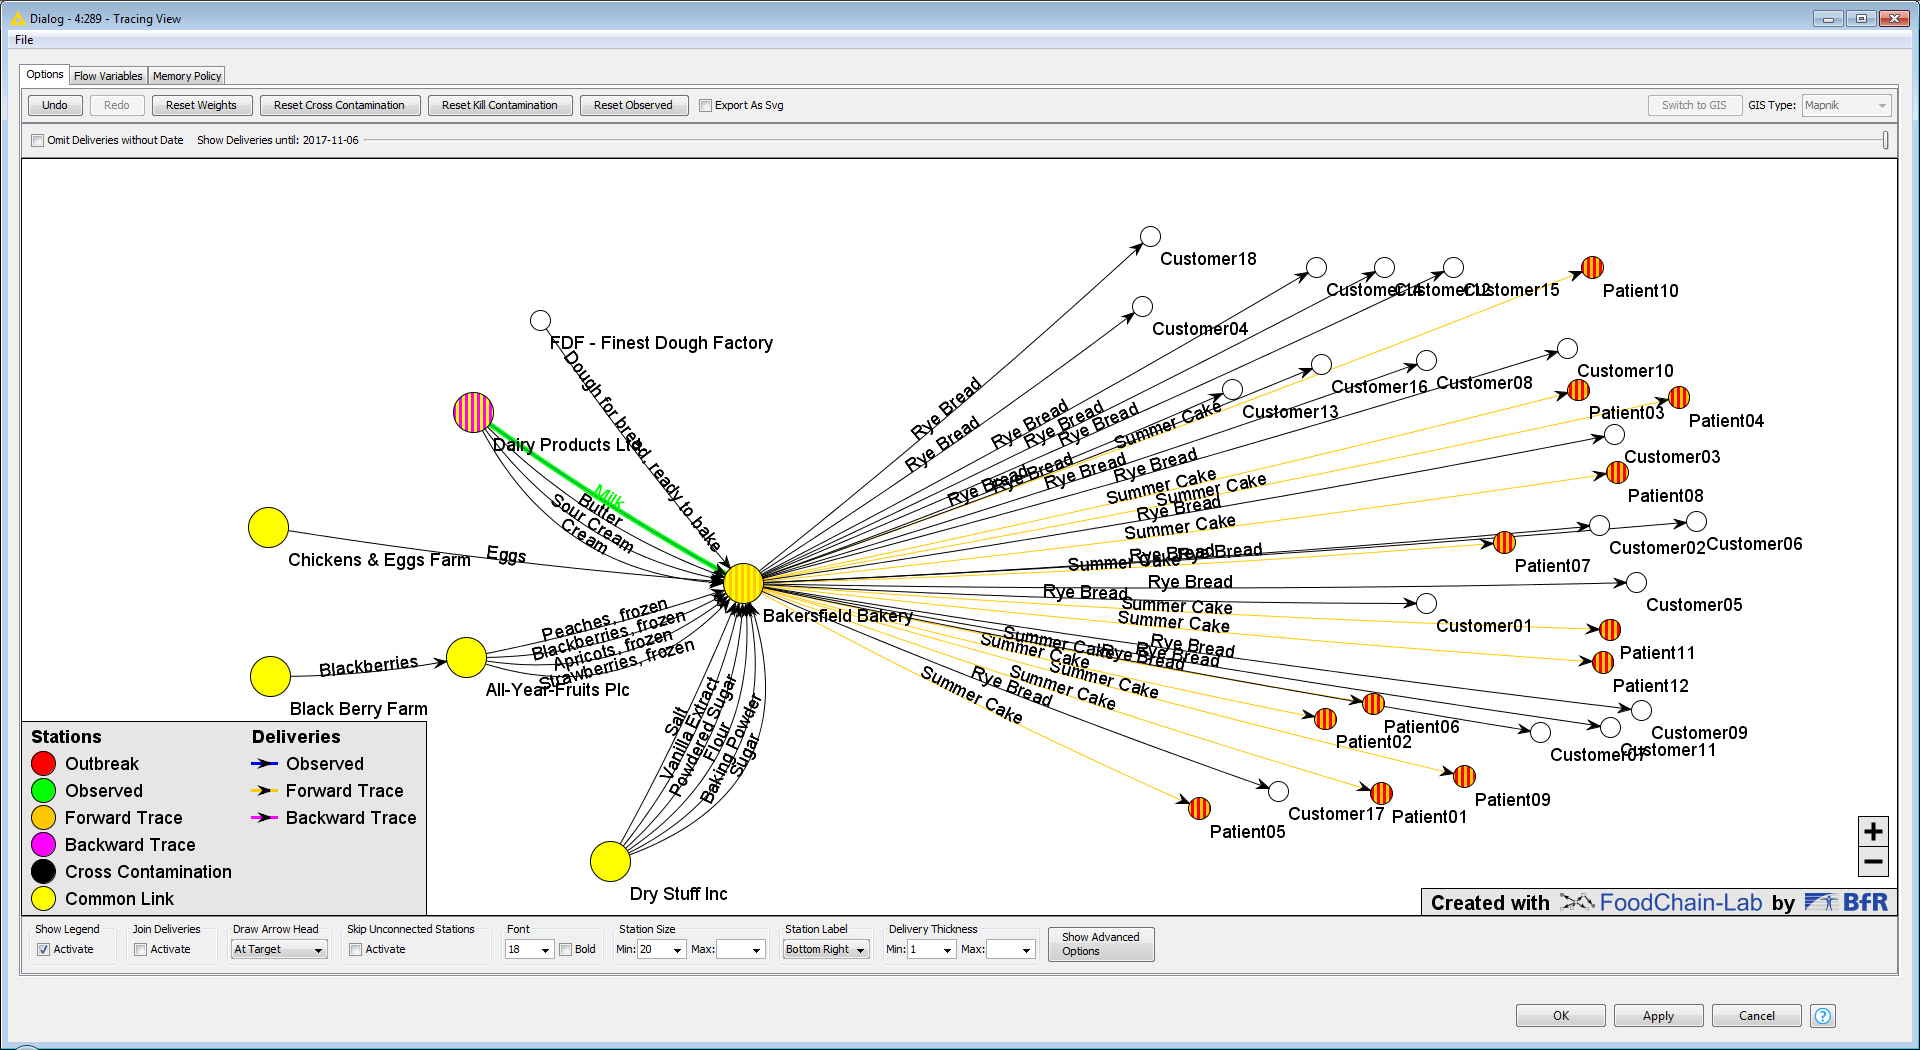
\includegraphics[height=0.6\textheight]{7b.png}
	\end{center}
	\begin{itemize}
		\item All of the outbreak stations (and these only) belong to the forward trace. You seem to have found the source of the outbreak: The milk pasteurizer in the company \textit{Dairy Products Ltd.} If only tracing was always this easy...
	\end{itemize}
	\end{frame}

\end{document}
